%!TEX root=../main.tex
\chapter{Climbing Mont Blanc Improvements}
\label{ch:improvements}

In this chapter it is assumed that a web interface follows the \gls{mvc} pattern. As briefly mentioned in sub-section \ref{subsec:cmb-arch-frontend}, Angular structures the HTML and Javascript code according to the \gls{mvc} pattern, and the reader should have the abstraction in mind when reading about browser or frontend implementations.

\section{Real Time Updates}
The frontend view changes when a user performes actions against the frontend models as mentioned in sub-section \ref{subsec:cmb-arch-frontend}. However, the frontend view presented to a given user does not update automatically as other users interract and changes their data models, as models is stored locally in each of the user's browser. If the updated model contains data that should be known\footnote{Hereby known as \textit{shared data}.} to all users, the users does not get notified about the model changes dynamically and views may therefore display out of date information. Figure \ref{fig:update-problem} shows an example of the problem, as Alice updates some of her browser's model data when she interacts with the system. If Alice changes some data present in Bob's models, Bob will not be notified of the changes as all data transfer are done with HTTP requests between Alice and the server. However, Bob can fetch up to date data by manually refreshing his webpage. \\

\begin{sidewaysfigure}
    \centering
    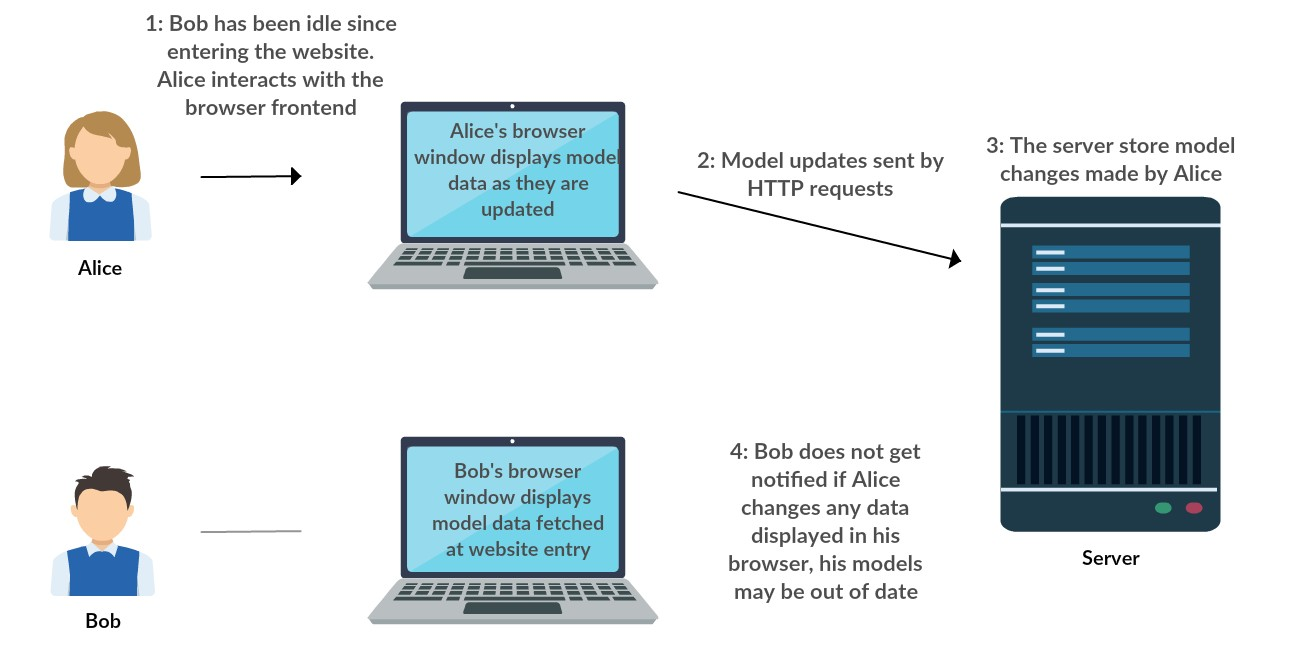
\includegraphics[width=1\textwidth]{figs/update_problem.jpg}
    \caption{Example of updating models without model change notifications}
    \label{fig:update-problem}
\end{sidewaysfigure}

Many websites requires to share data between multiple clients and dynamically notify clients if there are changes to the data. As an example in the \gls{cmb} system, it would be nice if the frontend interface dynamically updated as a user's submission finished running at the backend. In the old system before the improvements, the user had to manually refresh by clicking at a refresh button provided by the user interface or manually refresh the webpage. However, this section presents a technology which has been introduced in the new version of the system in order to dynamically update data relevant for multiple clients. \\

Socket.io \cite{SOCKETIO} is an \gls{api} for enabling real time communication between the server and connected clients. The \gls{api} was first made as Javascript library, but many open source projects have developed modules for other programming languages integrating the Socket.io \gls{api}. One benefit of the \gls{api} is that it works as a wrapper around a set of real time communication protocols to enable support for different browsers, which means that the framework can automatically detect the protocol supported by a client and use that information to select the best fitted communication protocol. \\

Rohit Rai states the communication protocols supported by the Socket.io \gls{api} \cite{Rai2013}. Figure \ref{fig:cmb-protocols} shows the communication protocols enabled in the new version of \gls{cmb}. The WebSocket protocol \cite{a:Fette2011}, shown in Figure \ref{fig:websocket}, has become more popular since its introduction in 2011 and is now supported by the most popular browsers. The protocol is a bit different from the well known HTTP protocol, as there is a persistent connection, or socket, between the client and the server as long as both entities are connected to the socket. The socket connection is closed if the client closes the browser window or the server goes down, or if the code explicitly indicates to close the socket. WebSockets enables easy two-way communication by letting two entities emit (read: send) messages back and forth on the socket connection, and respond differently depending on the type of message emitted on the socket. \\

Polling and long-polling are very similar as they both rely on the HTTP protocol. However, in long-polling, the server keeps the connection between the two entities open until there is an update to the requested data as shown in Figure \ref{fig:long-polling}. In polling, as shown in Figure \ref{fig:polling}, the client continuously requests data with some constant delay between each request, while the server respond on each request with the data currently stored at the server. Independent of the protocol, we as programmers can abstract away the connection and think of it as a "socket" connecting the client and the server. \\

\begin{figure}
    \centering
    \begin{subfigure}[b]{1.0\textwidth}
        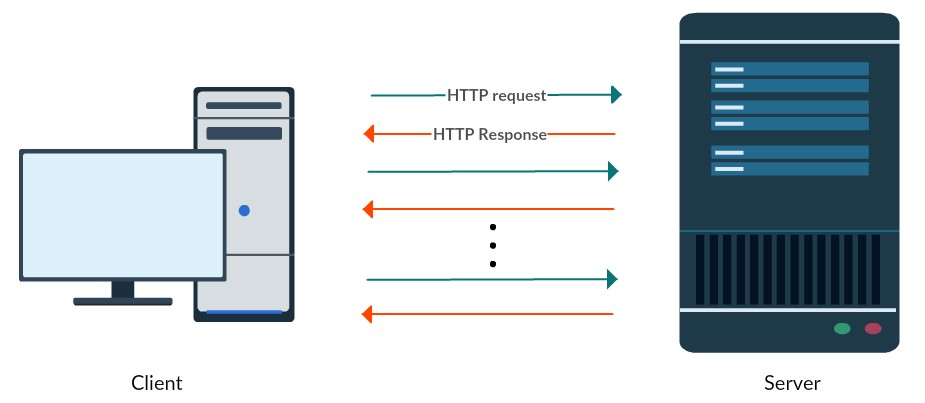
\includegraphics[width=\textwidth]{figs/polling.jpg}
        \caption{Polling: The client sends a series of HTTP request and the server responds on each request.}
        \label{fig:polling}
    \end{subfigure}
    ~ %add desired spacing between images, e. g. ~, \quad, \qquad, \hfill etc.
    %(or a blank line to force the subfigure onto a new line)
    \begin{subfigure}[b]{1.0\textwidth}
        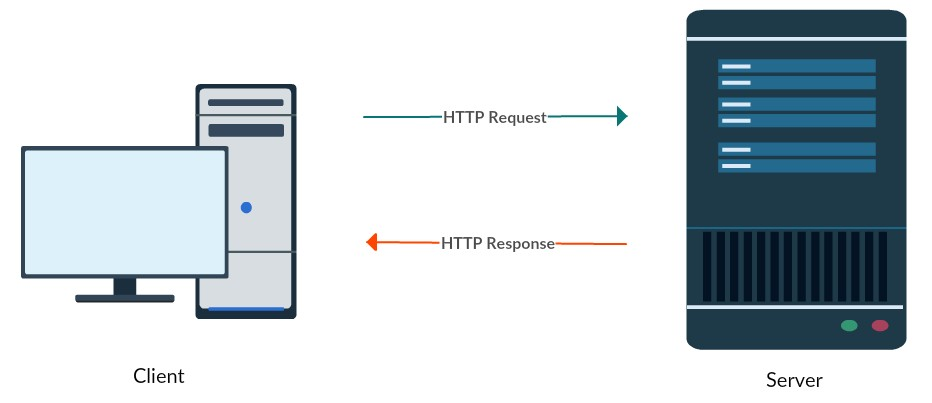
\includegraphics[width=\textwidth]{figs/long_polling.jpg}
        \caption{Long-polling: The client sends an HTTP request to fetch new data, the server holds the connection open until the requested data is updated.}
        \label{fig:long-polling}
    \end{subfigure}
    \begin{subfigure}[b]{1.0\textwidth}
        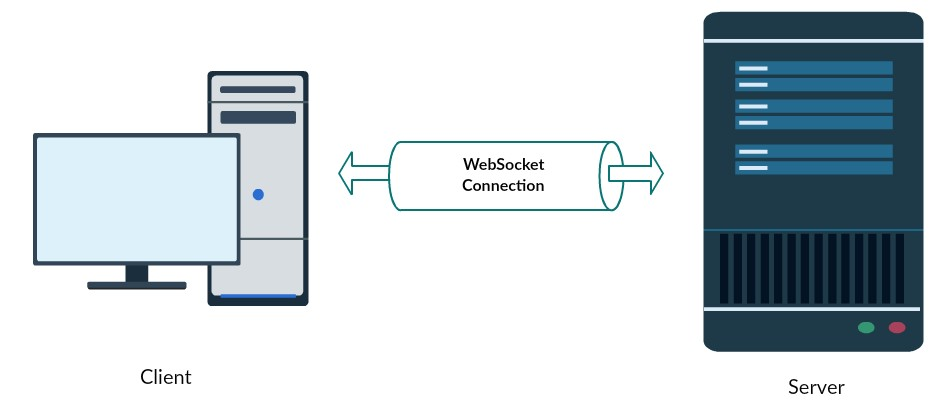
\includegraphics[width=\textwidth]{figs/websocket.jpg}
        \caption{WebSocket protocol: a two-way connection tunnel open throughout the whole client session. TCP is used as a transport protocol.}
        \label{fig:websocket}
    \end{subfigure}
    \caption{\gls{cmb} Socket.io communication protocols}\label{fig:cmb-protocols}
\end{figure}

Each socket can be "\textit{namespaced}" into separate communication channels within an application. A namespace can be viewed as a endpoint or network path, for example in the new \gls{cmb} prototype the namespace \textit{/cmb} is used as default namespace to emit messages between the client and the server. Every client initiating a socket on the namespace receives all messages emitted to the namespace, which makes it easy to share information between the server and clients connected to the namespace. \\

Each namespace can also define a set of \textit{rooms}, which can be viewed as sub-channels of a given namespace. A client needs to explicitly join a room to receive the messages emitted in the sub-channel. Figure \ref{} shows an example use case of rooms and namespaces in the new \gls{cmb} system. Socket.io also lets the programmer define \textit{events}, which can be emitted between the server and connected clients. Table \ref{} shows the events currently defined for the \gls{cmb}, and the actions taken either by the server or client depending on which entity that emitted the event. The two below sub-sections describes the technologies used by the server and frontend in order to support real time communication with Socket.io.

\subsection{Frontend Technology}
The frontend uses the client Socket.io library through a existing Socket.io component called \texttt{angular-socket-io} \cite{ANGULARSOCKETIO}.

\subsection{Server Technology}
The Python module Flask-SocketIO \cite{FLASKSOCKETIO} enables Flask applications to use the SocketIO \gls{api}. In addition, the modules gevent \cite{GEVENT} and gevent-websocket \cite{GEVENTWEBSOCKET} is installed in combination with the Socket.io module to enable the use of the WebSocket protocol. Gevent is a coroutine based networking library providing a high-level synchronous API on top of a asynchronous webserver. Asynchronous coroutines is used to handle multiple concurrent requests from multiple clients, and is required by the Flask-Socketio module to support the WebSocket transport. \\

To fully support the WebSocket protocol Gunicorn also needs to make use a custom gevent worker supporting the WebSocket protocol. As stated by Miguel Grinberg on the Flask-Socketio documentation website, Gunicorn can only enable one worker due to limitations in the implemented load balancing algorithm. The Gunicorn load balancing algorithm cannot simply handle multiple workers and persistent WebSockets connections, which limits us to one worker per server. However, the worker uses coroutines to handle multiple concurrent requests as stated above. The gevent worker is enabled on the development server of \gls{cmb}, which also required some changes to the Nginx setup to fully support the WebSocket protocol. Appendix \ref{apdx:setup} describes setup information necessary to setup servers with Gunicorn and Nginx, while section \ref{sec:eval-tech} discusses pros and cons with selected technologies as well as presenting alternatives to the selected technology stack.

\section{Frontend}
\subsection{Bug Fixes}
Upload fixes in frontend
Sorting bug

\subsection{Views and Feedback}
Spinners + better error messages. Bulletin board to display administrator messages. Colored feedback messages.

\subsection{Group Functionality Improvements}
Gathered group functionality. JSON stat file download.

\section{Server}

\subsection{Database Management System}
SQLAlchemy MYSQL adapter + possible async library.

\subsection{Database Model Updates}
Detailed state field added and can be replaced with json structures as more information is needed about a run.
Bulletins table added. Cascading delete.

\subsection{Admin Interface}
Several new problems have been added to the system during the Spring semester. Most problems were added due to a master thesis of two students, assessing the \gls{cmb} system's suitability for conducting digital exams in the course TDT4102 Procedural and Object-Oriented Programming \cite{TDT4102}. However, many of the
Bug fix: Unix vs DOS files. Delete files in file system after model is deleted in the database.


\section{Backend}
There have been some small changes in the backend code. The \gls{cmb} team discovered that there were no timeout when running the small correctness test, which could potentially lock the backend if the submitted code contained infinite loops. Locking the backend should not be acceptable under any condition, and the Unix program \texttt{timeout} \cite{TIMEOUT} is therefore used as during the big correctness test to kill the submitted program after some time if it stalls to long. Since the small input set is much smaller than the big correctness test, it is currently set to a third of the timeout of the big correctness or 30 seconds. \\

The \gls{json} returned by the backend is also slightly changed. A "state" field were added to better track the state of the program as it executes on the backend, especially if there is an error during execution. The field is currently used as input to the "detailed state" database field as described above, which is further used in the frontend to specialize the feedback given to the user if there is an error during execution of the program. Currently, the field is a simple string describing the state of the submitted program when the backend are done executing. A quick further discussion of the field and its potential are described in section \ref{sec:eval-tech}.

\section{Improvement Proposals}
